\chapter{Image Embedding}
\label{ch:image-embedding}

Every data set so far came in the matrix (tabular) form: objects (say, tissue samples, students, flowers) were described by row vectors representing a number of features. Not all the data is like this; think about collections of text articles, nucleotide sequences, voice recordings or images. \marginnote{This depiction of deep learning network was borrowed from \url{http://www.amax.com/blog/?p=804}}It would be great if we could represent them in the same matrix format we have used so far. We would turn collections of, say, images, into matrices and explore them with the familiar prediction or clustering techniques.

\begin{wrapfigure}{o}{1.0\textwidth}
    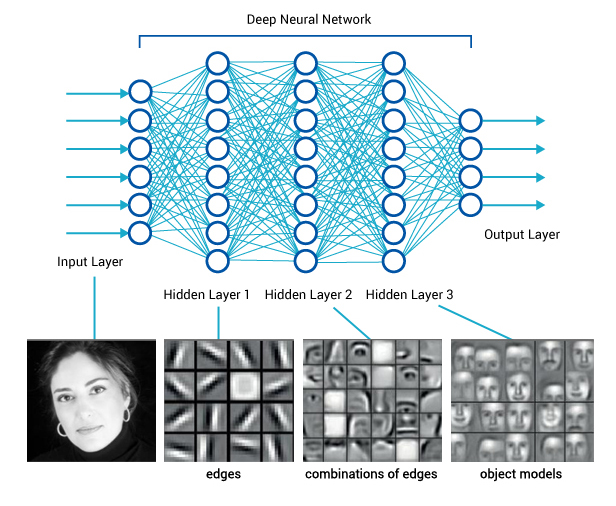
\includegraphics[scale=0.5]{blog_deeplearning.jpg}
    \label{fig:deep-learning}
\end{wrapfigure}

Until very recently, finding useful representation of complex objects such as images was a real pain. Now, technology called deep learning is used to develop models that transform complex objects to vectors of numbers.

Consider images. When we, humans, see an image, our neural networks go from pixels, to spots, to patches, and to some higher order representations like squares, triangles, frames, all the way to representation of complex objects. Artificial neural networks used for deep learning emulate these through layers of computational units (essentially, logistic regression models and some other stuff we will ignore here). If we put an image to an input of such a network and collect the outputs from the higher levels, we get vectors containing an abstraction of the image. This is called embedding.

\begin{wrapfigure}{o}{0.8\textwidth}
    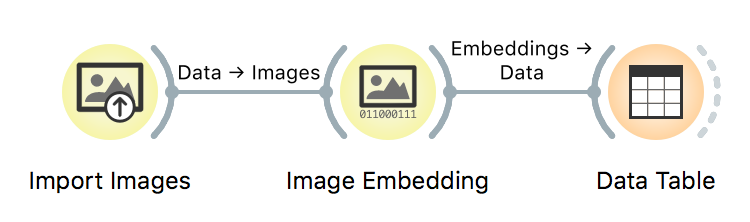
\includegraphics[scale=0.6]{workflow-embedding.png}
    \label{fig:embedding}
\end{wrapfigure}

Deep learning requires a lot of data (thousands, possibly millions of data instances) and processing power to prepare the network. We will use one which is already prepared. Even so, embedding takes time, so Orange doesn't do it locally but uses a server invoked through the \widget{Image Embedding} widget.

\newpage

Image embedding describes the images with a set of 2048 features appended to the table with meta features of images.

\begin{figure*}[h]
    \centering
    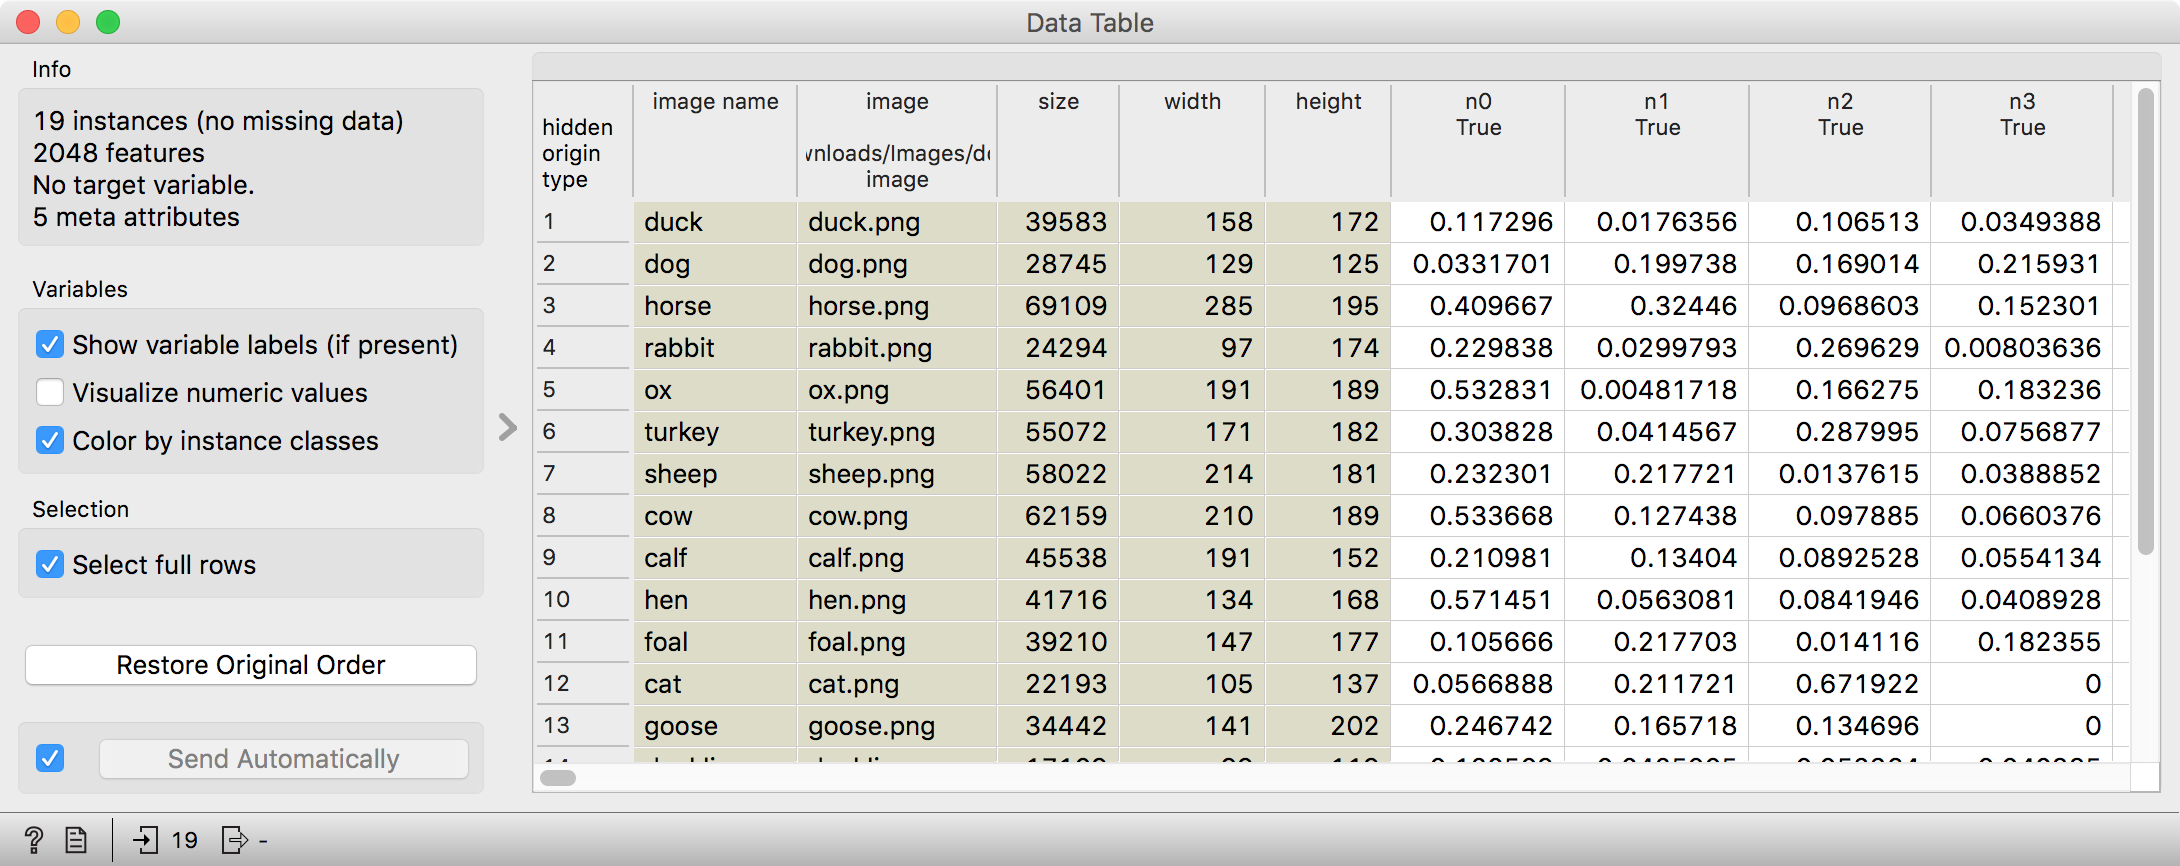
\includegraphics[scale=0.45]{data-table.png}
    \caption{$\;$}
\end{figure*}

We have no idea what these features are, except that they represent some higher-abstraction concepts in the deep neural network (ok, this is not very helpful in terms of interpretation). Yet, we have just described images with vectors that we can compare and measure their similarities and distances. Distances? Right, we could do clustering. Let's cluster the images of animals and see what happens.

\begin{figure*}[h]
    \centering
    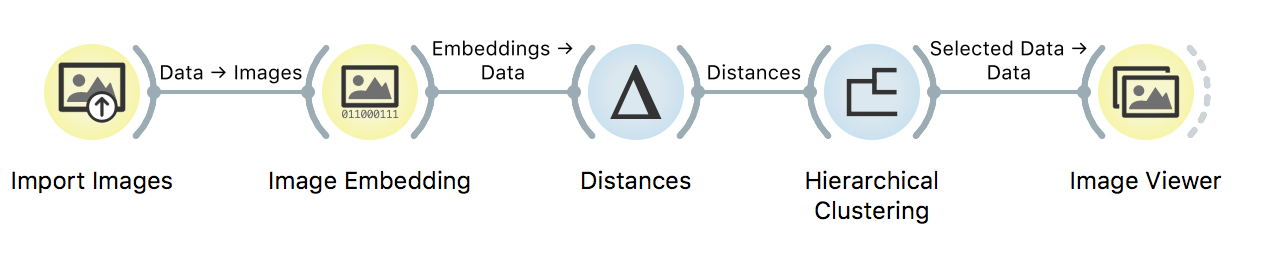
\includegraphics[scale=0.6]{workflow-clustering.png}
    \caption{$\;$}
\end{figure*}

To recap: in the workflow above we have loaded the images from the local disk, turned them into numbers, computed the distance matrix containing distances between all pairs of images, used the distances for hierarchical clustering, and displayed the images that correspond to the selected branch of the dendrogram in the \widget{Image Viewer}. We used cosine similarity to assess the distances (simply because the dendrogram looked better than with the Euclidean distance).

\begin{marginfigure}
    \centering
    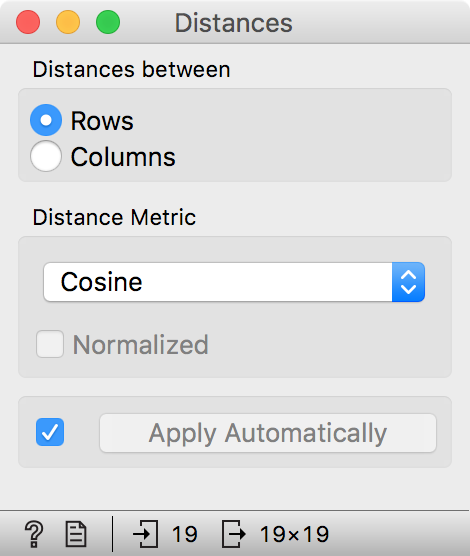
\includegraphics[scale=0.6]{distances.png}
    \caption{$\;$}
\end{marginfigure}

\newpage

Even the lecturers of this course were surprised at the result. Beautiful!

\begin{figure*}[h!]
    \centering
    \newcommand{\hierclust}{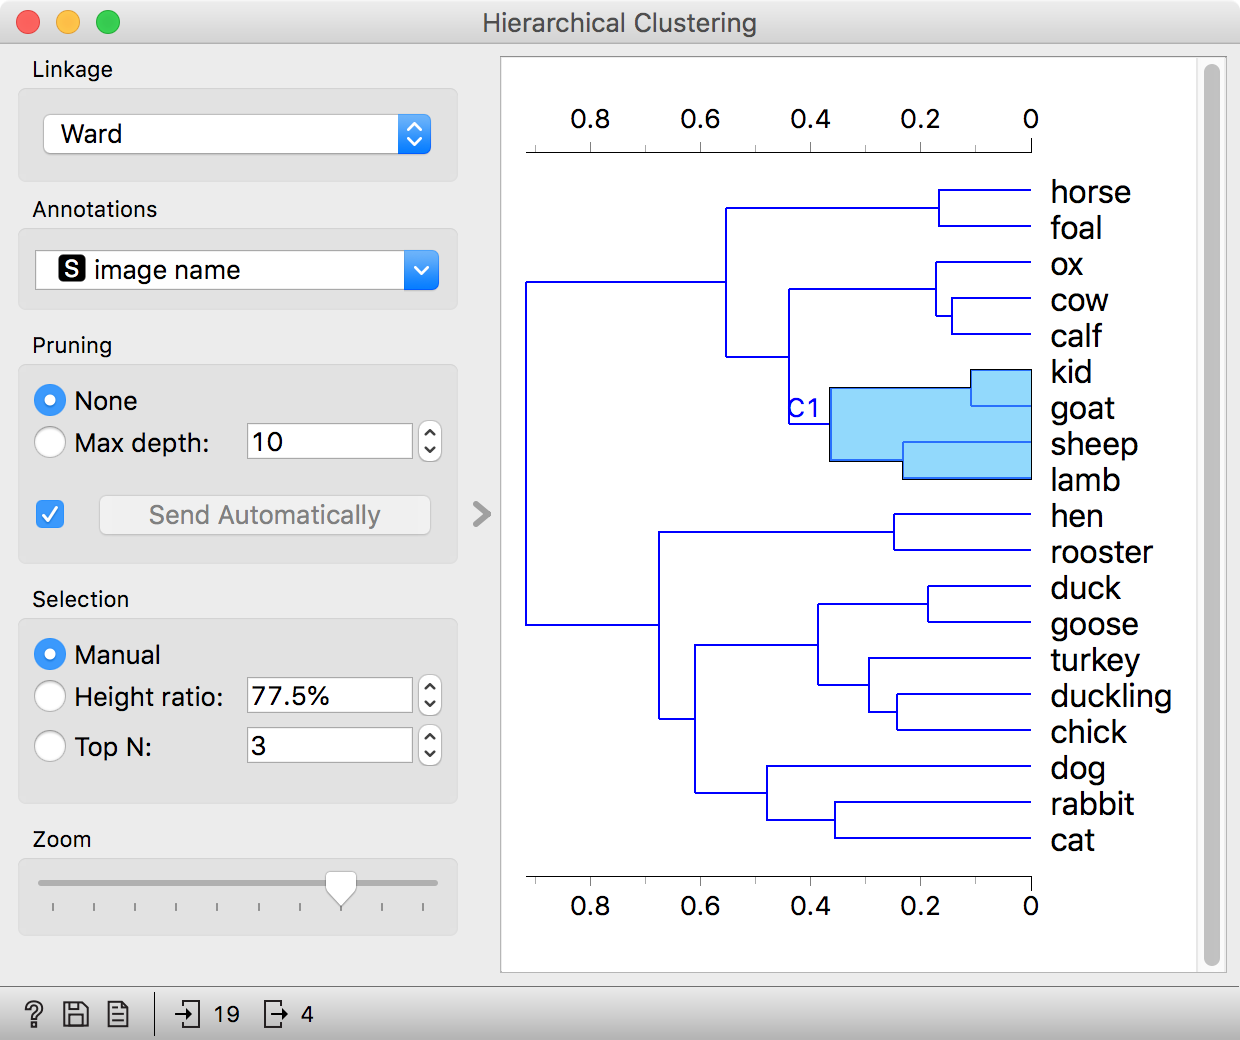
\includegraphics[scale=0.45]{hier-clustering.png}}
    \newcommand{\imageview}{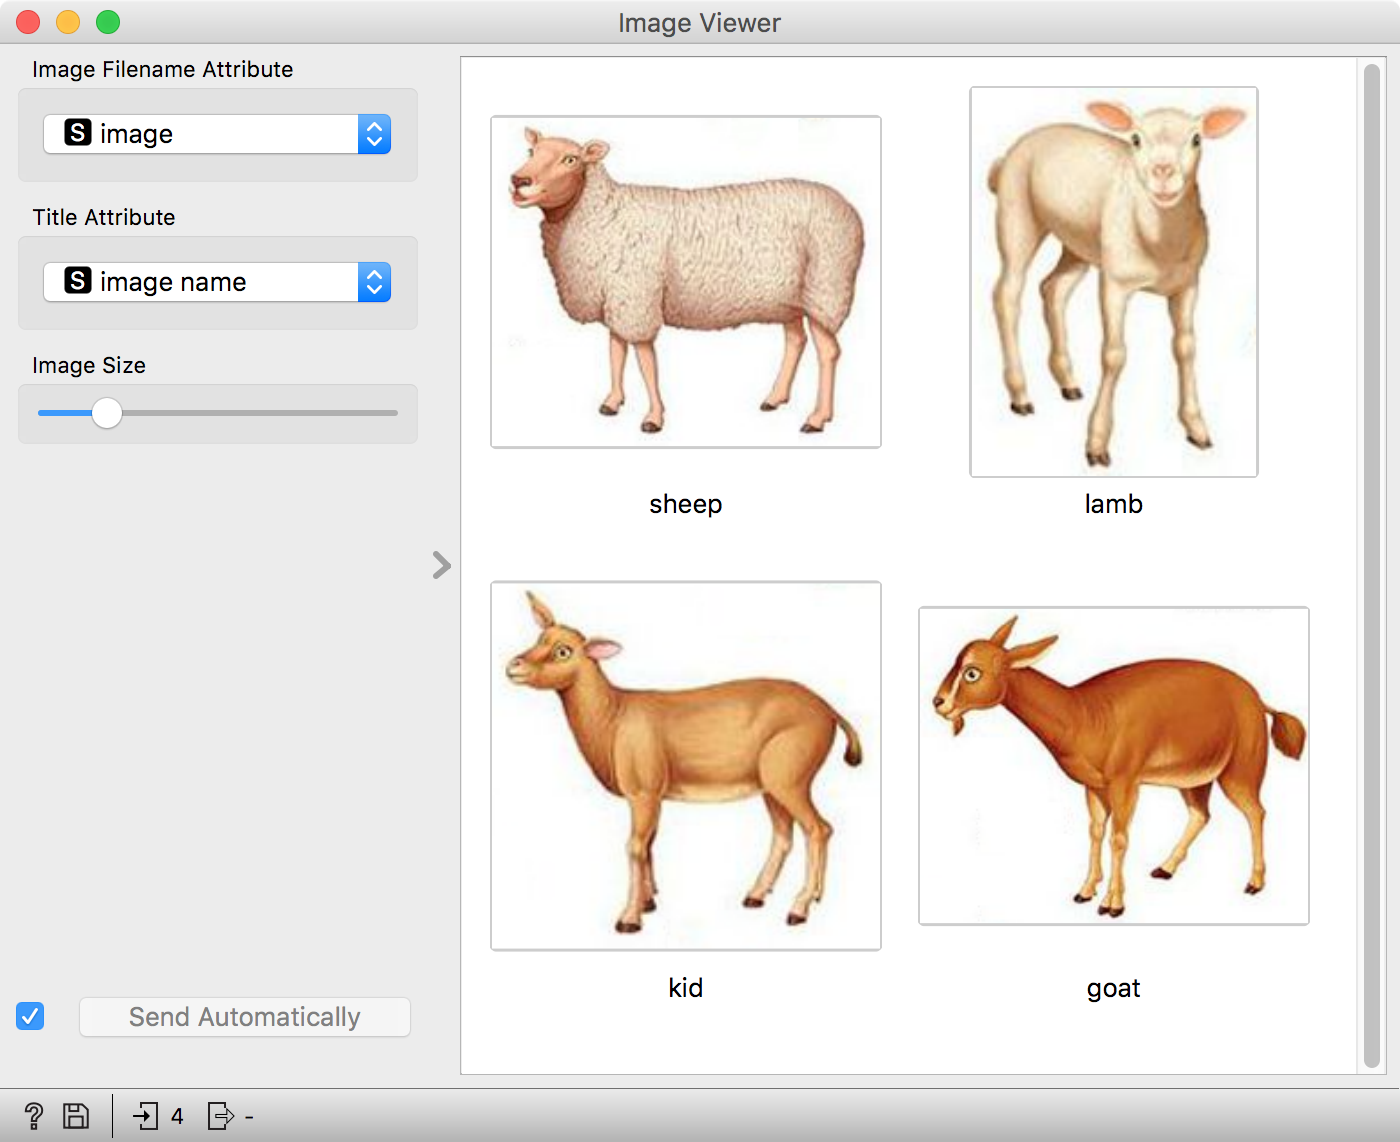
\includegraphics[scale=0.45]{image-viewer.png}}
    \infinitewidthbox{
    \stackinset{r}{-0.35\linewidth}{t}{+0.45\linewidth}{\imageview}{\hierclust}\hspace{6cm}
    }
\end{figure*}
